\chapter{Analysis of the depth data}
\label{cha:analysis}

The acquired depth information is stored in computer memory in two ways. The first is a depth map, which takes the form of a two dimensional array, similarly to a plain gray-scale image. In this case, however, the depth measurement is stored in place of the color intensity. Depth map is the simplest way to represent and store the acquired depth of the scene and it is usually obtained directly from the sensor driver. The main disadvantage of a depth map is its inflexibility. This representation is strictly bound to the camera point of view and, thus, it is inconvenient in further processing. 

The second representation of a scene's depth information is a point cloud. Generally speaking, it is a set of data points in some coordinate system. The Cartesian system is typically used and the points are defined by their x, y and z coordinates. Point clouds are derived from depth maps and offer new capabilities, such as viewpoint transformation or cloud concatenation. The point cloud representation can be rendered in the three dimensional space, which is a particularly useful tool during the implementation of the system for depth data analysis. 


In order to achieve the autonomous operation of the robot, a set of tools for efficient processing and analysis of the collected data about the environment structure must be established. The following sections present the main operations used further in the implementation of the autonomous control mode for the MMS robot.



%---------------------------------------------------------------------------

\section{Basic point cloud processing}
\label{sec:pointclouds}

In a given point cloud, a single point by itself does not provide much information about the surface to analyse. Therefore, an essential concept in depth data analysis is the local neighbourhood of a point. For a query point $p_q$ in the point cloud $P$ its neighbourhood is given by:
\begin{equation}
d(p_	q, p_i) \leq r
\end{equation}
where $p_i \in P$ is the neighbouring point, $d$ is the selected metric, typically Euclidean, and $r>0$ is the neighbourhood radius. In practice, approximate methods are used, as direct application of the definition would require calculation of distance from the query point $p_q$ to all other points in $P$. The algorithms used for neighbourhood search require a parameter $k$ specifying the maximum number of points in the neighbourhood or parameter $r$, denoting the maximum search radius. Proper determination of those parameters is crucial in further analysis. Too small values will not provide enough information about the surface. Too large, on the other hand, will average the surface and skip small details.

A frequently used operation during the processing of a point cloud is the affine transformation. Point clouds can be translated, rotated and scaled by multiplying a transformation matrix $A \in \mathbb{R}^{4x4}$ with data points in homogeneous coordinates $[x,y,z,1]^T$. Basic transformation matrices are demonstrated in the Figure \ref{fig:transformations}. Presented transformations can be further combined by multiplication to produce more complex operations.

\begin{figure}[H]  

  \begin{minipage}{.3\linewidth}
    \centering
    \[A_t=\left[\begin{array}{cccc}
      1 & 0 & 0 & t_x \\
      0 & 1 & 0 & t_y \\
      0 & 0 & 1 & t_z \\
      0 & 0 & 0 & 1
    \end{array}\right]\]
    Translation by a vector $t=[t_x,t_y,t_z]^T$
  \end{minipage}%
  \begin{minipage}{.3\linewidth}
    \centering
    \[A_s=\left[\begin{array}{cccc}
      S_x & 0 & 0 & 0 \\
      0 & S_y & 0 & 0 \\
      0 & 0 & S_z & 0 \\
      0 & 0 & 0 & 1
    \end{array}\right]\]
    Scaling along $x,y,z$ by factors $S_x,S_y,S_z$
  \end{minipage}  
  \begin{minipage}{.4\linewidth}
    \centering
    \[A_x=\left[\begin{array}{cccc}
      1 & 0 & 0 & 0 \\
      0 & cos(\theta_x) & -sin(\theta_x) & 0 \\
      0 & sin(\theta_x) & cos(\theta_x) & 0 \\
      0 & 0 & 0 & 1
    \end{array}\right]\]
    Rotation around $x$ with \\ $\theta_x$ angle
  \end{minipage}%
  
  \begin{minipage}{.5\linewidth}
    \centering
    \[A_y=\left[\begin{array}{cccc}
      cos(\theta_y) & 0 & sin(\theta_y) & 0 \\
      0 & 1 & 0 & 0 \\
      -sin(\theta_y) & 0 & cos(\theta_y) & 0 \\
      0 & 0 & 0 & 1
    \end{array}\right]\]
    Rotation around $y$ with $\theta_y$ angle 
  \end{minipage}
  \begin{minipage}{.5\linewidth}
    \centering
    \[A_z=\left[\begin{array}{cccc}
      cos(\theta_z) & -sin(\theta_z) & 0 & 0 \\
      sin(\theta_z) & cos(\theta_z) & 0 & 0 \\
      0 & 0 & 1 & 0 \\
      0 & 0 & 0 & 1
    \end{array}\right]\]
    Rotation around $z$ with $\theta_z$ angle 
  \end{minipage}
  
  
  \caption{Basic affine transformations}
  \label{fig:transformations}
\end{figure}

%Info from pcl tutorials.

 One of the most important stages of data preprocessing is the filtration. Probably the most basic point cloud filter is the pass-through filter, which reject all points outside a given range along a specified dimension. This procedure allows to focus the analysis process on the region of interest, i.e. the reachable workspace of a manipulator. Apart from limiting the cloud dimensions, the number of data points can be also reduced by downsampling. The voxel grid filter is typically used for this purpose. This filter creates a three dimensional regular grid over the input point cloud data and then, in each voxel, approximates all the present data points with their centroid. Such reduction is particularly useful when large point cloud datasets have to be processed online with limited computing resources. Finally, the filtration process has to cope with numerous measurement errors present in the raw data acquired from the 3D camera. Such measurement noise 
manifests itself in the form of sparse outliers, which corrupt the results of further processing, i.e. the surface normals estimation. The impact of those irregularities can by reduced by applying an outlier removal filter. The simplest form of such filter rejects all the data points which does not have enough neighbours within a specified radius. A more refined version is based on the neighbouring points distance distribution. Firstly, the mean distance from each point to all its neighbours is calculated. Next, based on the assumption that the resulting distribution is Gaussian, all the points whose mean distances lay outside of an interval defined by the global distances mean and their standard deviation are rejected from the dataset. The effects of statistical outlier removal are presented in the Figure \ref{fig:outlierremoval}.

The point cloud segmentation or cluster extraction is the process of grouping together data points that meet some common condition of similarity. Ideally, each of such segmented clusters represents a different object in the scene. A popular segmentation method is based on the euclidean distance. In this approach, two points are considered to belong to the same cluster, if their relative distance is less than a selected threshold. This process is similar to the flood-fill algorithm, popular in the 2D image processing. There are also other varieties of segmentation, i.e. based on the smoothness constraint or colour similarity.

\begin{figure}[H]
\centering
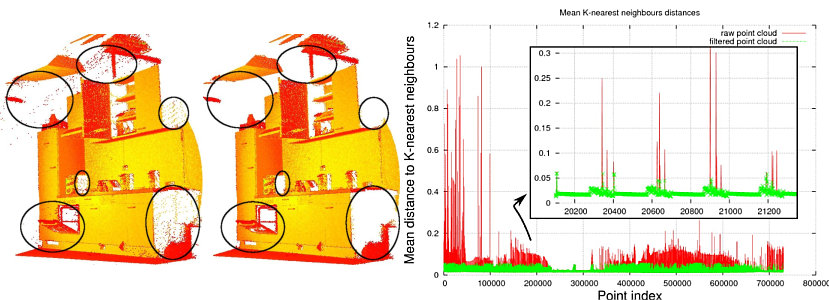
\includegraphics[width=0.9\textwidth]{fig/statistical_removal}
\caption{Statistical outlier removal \cite{pcl}}
\label{fig:outlierremoval}
\end{figure}

%Info from Rusu dissertation

Many of the algorithms used further during the analysis of a point cloud base on the notion of a surface normal, known from the 3D geometry. These vectors are also widely used for shading in 3D computer graphics and a variety of methods have already been developed to solve the surface normal estimation problem. One of the simplest uses the least-squares plane fitting to estimate the normal to a plane tangent to the surface, which approximates the desired vector \cite{rusuthesis}. More specifically, for a given point on the surface, it's $k$-neighbourhood centroid $\bar{p}$ is calculated as:
\begin{equation} 
\bar{p} = \frac{1}{k} \cdot \sum\limits_{i=1}^{k} p_i 
\end{equation}
The tangent plane is thereafter defined by the centroid $\bar{p}$ and the sought normal vector $\vec{n}$. The latter is computed by minimizing the total distance from every k-neighbour $p_i$ to the tangent plane, given by $\sum\limits_{i=1}^{k} (p_i - \bar{p})\cdot \vec{n}$. The minimization problem can be solved by utilizing the covariance matrix $C \in \mathbb{R}^{3x3}$, given by:
\begin{equation}
C = \frac{1}{k}\sum\limits_{i=1}^{k}(p_i - \bar{p})\cdot (p_i - \bar{p})^\intercal
\end{equation}
The covariance matrix $C$ is symmetric, positive semi-definite and possess three real eigenvalues $\lambda_j \geq 0, i = 1,2,3$. The eigenvector corresponding to the smallest eigenvalue is an approximation of the desired normal vector $\vec{n}$, disregarding the sign. Furthermore, if the viewpoint $v_p$ is known, the normal $\vec{n}$ has to be oriented towards  $v_p$, which means that it has to satisfy the condition:
\begin{equation}
\vec{n}\cdot(v_p-p_i) > 0
\end{equation}
%---------------------------------------------------------------------------

\section{The Random Sample Consensus algorithm}
\label{sec:ransac}
The indoor human environment is abundant of regularly shaped objects that could be described with basic geometrical models, such as planes, spheres or cylinders. The plane model:
\begin{equation}
A \cdot x+ B \cdot y+ C \cdot z+ D= 0
\label{eq:planemodel}
\end{equation}
is particularly useful, as the floor, walls or the furniture is typically composed of flat surfaces. In example, by knowing which points of the scene belong to the surface of a floor, the robot can autonomously plan a collision-free path of movement. For this reason, a robust model fitting algorithm is a strongly desired tool in the analysis of the depth data. The point dataset received from the depth camera, however, consists of both points that belong to the model, the inliers, and a lot of other points in the scene, the outliers. Therefore direct usage of classic model fitting algorithms, such as the least squares method, would not provide the desired effect, as they try to fit the model into all the input data points, including outliers. As an alternative, the Random Sample Consensus (RANSAC) algorithm, can effectively cope with such problems. In its basic form, the RANSAC algorithm is essentially composed of two, iteratively repeated steps \cite{wikipedia,ransacdummies}:
\begin{enumerate}
\item Firstly, a minimal sample subset is randomly selected from the input dataset. The model parameters are computed using only the selected subset. The cardinality of the subset is the smallest sufficient to determine the model parameters.
\item Secondly, the remaining dataset points are tested to be consistent with the model computed in the sampling step. A data point will be considered as an inlier if it fits the computed model within a defined error threshold. The set of such elements is called a consensus set. If the consensus set contains enough points, the model is reestimated from all selected inliers and evaluated with the error of the inliers relative to the model.
\end{enumerate}
This procedure is then repeated until a termination condition is met, which usually is a fixed number of iterations.
The main advantage of the RANSAC algorithm is its robust estimation. This method is able to fit a model with high accuracy even if the data set contains a significant amount of outliers. On the other hand, the algorithm in its basic form has several disadvantages. There is no upper bound on the time needed to estimate model parameters and by limiting the number of iterations, the obtained solution is may not be optimal. Furthermore, the RANSAC algorithm can only estimate one model per dataset and if multiple models exist, it may fail to estimate any of them. Since the original RANSAC was first published in 1981, it has been widely adapted by the image processing community and many modifications that address the RANSAC limitations has been proposed. A comparative summary of the recent extensions to the RANSAC algorithm can be found for example in \cite{ransacsurvey}.



%---------------------------------------------------------------------------

\section{Descriptors for object recognition}
\label{sec:descriptors}

The object recognition, which involves the identification and localization of a given 3D object in the environment, is a major problem and limitation during the execution of autonomous manipulation tasks. Most of the 3D recognition methods base on some surface characteristics indicators, called features or descriptors. Surface normals are the most basic representation of the geometry around a certain point. Even if coupled with surface curvature, they usually does not provide enough descriptive information for object recognition and pose estimation. To achieve better performance in such tasks, more complex and higher dimensional descriptors have been proposed in the literature \cite{descriptorssummary}. A descriptor is considered to be reliable if it is able to capture the same surface characteristics, regardless of rigid transformations, varying sampling density and noise. In general, 3D shape descriptors are divided into local and global. The former describe only the local geometry around a query point, while the latter represent the geometry of the whole object. A few selected descriptors are presented further in this section.

The Point Feature Histogram (PFH) \cite{rusuthesis} is a generalization of both surface normals and curvature estimates. It represents the relative orientation of normals between every point pair $(p_i,p_j)$ in the neighbourhood of the query point $p_q$. For each point pair, using the surface normal $n_i$ at $p_i$, a new coordinate frame $u,v,w$ is constructed as follows:
\begin{equation}
u = n_i,\  v = u \times \frac{p_i-p_j}{d},\  w = u \times v
\end{equation}
where $d = \|p_i-p_j\|_2$ is the Euclidean distance between $p_i$ and $p_j$. Using this reference frame, the difference between normals at $p_i$ and $p_j$ is expressed by the angular features $\alpha, \phi, \theta$, given by:
\begin{equation}
\alpha = v \cdot n_i, \  \phi = u \cdot \frac{(p_i-p_j)}{d}, \ \theta = arctan(w\cdot n_i, u \cdot n_i)
\label{eq:angularfeat}
\end{equation}
Finally, to create the PFH descriptor, the angular features are binned into a histogram. The angular ranges are typically divided into 5 subdivisions, thus receiving a $3^5=125$ binned histogram, that counts occurrences of any value combination for every point pair $(p_i, p_j)$.

The main disadvantage of the PFH descriptor is its $O(nk^2)$ complexity, where $n$ is the number of points in the point cloud and $k$ is the number of each points neighbours. For large datasets, this is one of the major bottlenecks during online processing. To overcome this problem a simplification to the PFH formulation, called Fast Point Feature Histogram has been proposed (FPFH) \cite{rusufpfg}. In the first step of the FPFH, the angular features $\alpha, \phi, \theta$ are computed only between the query point $p_q$ and its k-nearest neighbours, as described in Equation \ref{eq:angularfeat}. Those features produce a histogram, called Simplified Point Feature Histogram (SPFH). The SPFH is computed for every point in the cloud, and then, the FPFH descriptor is formed as follows:
\begin{equation}
FPFH(p_q) = SPFH(p_q) + \frac{1}{k}\sum\limits_{i=1}^k\frac{1}{w_i}SPFH(i)
\end{equation}
where $w_i$ is a distance between $p_q$ and $p_k$ in some metric space. The FPFH descriptor reduces the computational complexity of the PFH to $O(nk)$, while maintaining similar descriptive performance.


A further extension of the FPFH descriptor is the Viewpoint Feature Histogram (VFH). It is a global type of descriptor, resulting in only one histogram for a given cloud. The VFH utilises the viewpoint $p_v$ vector direction to add viewpoint variance to the FPFH. In this case, the angles $\alpha, \phi, \theta$ from \ref{eq:angularfeat} are computed between the entire point cloud centroid $p_c$ and each of the points and binned into a histogram. This signature is further extended by a viewpoint component - a histogram of the angles between each of the points and the normalized viewpoint direction vector $\frac{p_c - p_v}{\|p_c - p_v\|}$. The main advantage of the VFH is its computational efficiency, with complexity of $O(n)$. Furthermore, this descriptor encodes the objects surface within a single histogram, which makes it convenient to test for similarity between the given point clusters.
%PFH, FPFH, SHOT,	Keypoint extraction, VFH




%---------------------------------------------------------------------------

\section{Object recognition pipeline}
\label{sec:pipeline}

After computing the descriptors of the input cloud, the task of object recognition can be accomplished by matching  them with some classified training set. This training set is obtained on the basis of a object model, acquired i.e. by 3D scanning in a controlled environment. The local and global descriptors require two distinct approaches to the training model fitting procedure. The Figure \ref{fig:objpipe} presents complete processing pipelines for both types of descriptors, as proposed in \cite{AldomaMTWPZRGV12}.

\begin{figure}[H]
\begin{center}
\begin{tikzpicture}
  [node distance = 5mm,auto,every node/.style={rectangle,draw,align=center, font=\footnotesize}]
  
  \node (kpextr) at (1,10) {Key Point \\ Extraction};
  \node[right=of kpextr] (descr1) {Description};
  \node[right=of descr1] (match1) {Matching};
  \node[draw=none,fill=none, node distance=2mm, above=of match1](ann1) {\small Recognition Pipeline for Local Descriptors};
  \node[right=of match1] (corr) {Correspondence \\ Grouping};
  \node[right=of corr] (absor) {Absolute \\ Orientation};
  \node[below right=of absor] (icp) {ICP \\ Refinement};
  \node[right=of icp] (verify) {Hypothesis \\ Verification};
  \node[below left=of icp] (align) {Alignment};
  \node[left=of align] (match2) {Matching};
  \node[left=of match2] (descr2) {Desription};
  \node[left=of descr2] (segm) {Segmentation};
  \node[draw=none,fill=none, node distance=2cm, below=of ann1](ann2) {\small Recognition Pipeline for Global Descriptors};


  \foreach \from/\to in {kpextr/descr1,descr1/match1, match1/corr, corr/absor, absor/icp, icp/verify, segm/descr2, descr2/match2, match2/align, align/icp}
    \draw[->] (\from) -- (\to);

\end{tikzpicture}

\caption{Object recognition pipeline \cite{AldomaMTWPZRGV12}}

\label{fig:objpipe}

\end{center}
\end{figure}

In case of the local descriptors, the first stage of processing, is the extraction of key-points, that are characteristic points in which the features are further computed. The simplest approach to this step is to just downsample the input data, i.e. by a voxel grid filter. For the selected points, the local descriptors are then computed and matched with their closest correspondences in the training set, which results in a set of correspondence pairs. In the next phase, those pairs are grouped according to the geometric constrains of a rigid transformation and too small subsets are discarded. Two point pairs $(p_i, q_i)$ and $(p_j, q_j)$ are considered to be geometrically consistent, if, i.e., they meet the following relation:
$$ \left|\left\|p_i - p_j\|_2-\|q_i - q_j\right\|_2\right| < \epsilon $$
where $p$ and $q$ represent the model and the scene points, and $\epsilon$ is a given threshold. By applying the grouping step, a large number of the false correspondences is discarded. To finalize the recognition process, the transformation matrix parameters are estimated, i.e. using the RANSAC algorithm, to further reduce the number of inconsistent correspondences and return the absolute orientation of the object.

As it comes to global descriptors, the whole process is preceded by a segmentation phase, in order to extract individual objects in the scene. Next, for each cluster, a global descriptor is computed and compared to the training set elements, from which its closest neighbours are selected. The position of the object is then obtained by aligning the clusters centroids and the viewpoint information encoded in the descriptors.

The final two post-processing steps of both pipelines are intended to refine the recognition outcome. By applying the Iterative Closest Point (ICP) algorithm, which minimises the difference between two point clouds \cite{wikipedia}, the accuracy of the object position and orientation is improved. The hypothesis verification step aims to reduce the number of false positives of recognition. An example strategy for this step is presented in \cite{hipoveri} and is based on the number of inliers in the recognised cluster. 